\subchapter{Bootloader - U-Boot}{Objectives: Set up serial
  communication, compile and install the U-Boot bootloader, use basic
  U-Boot commands, set up TFTP communication with the development
  workstation.}

As the bootloader is the first piece of software executed by a
hardware platform, the installation procedure of the bootloader is
very specific to the hardware platform. There are usually two cases:

\begin{itemize}

\item The processor offers nothing to ease the installation of the
  bootloader, in which case the JTAG has to be used to initialize
  flash storage and write the bootloader code to flash. Detailed
  knowledge of the hardware is of course required to perform these
  operations.

\item The processor offers a monitor, implemented in ROM, and through
  which access to the memories is made easier.

\end{itemize}

The AM3358 SoC on the BeagleBone falls into the second category. The monitor
integrated in the ROM reads the SD card to search for a valid
bootloader.

Go to the \code{$HOME/__SESSION_NAME__-labs/bootloader} directory.

\section{Setting up serial communication with the board}

The Beaglebone serial connector is exported on the 6 pins close to one
of the 48 pins headers. Using your special USB to Serial adapter provided
by your instructor, connect the ground wire (blue) to the pin closest
to the power supply connector (let's call it pin 1), and the \code{TX} (red)
and \code{RX} (green) wires to the pins 4 (board \code{RX}) and
5 (board \code{TX})\footnote{See
\url{https://www.olimex.com/Products/Components/Cables/USB-Serial-Cable/USB-Serial-Cable-F/}
for details about the USB to Serial adapter that we are using.}.

You always should make sure that you connect the \code{TX} pin of the cable
to the \code{RX} pin of the board, and vice versa, whatever the board and
cables that you use.

\begin{center}
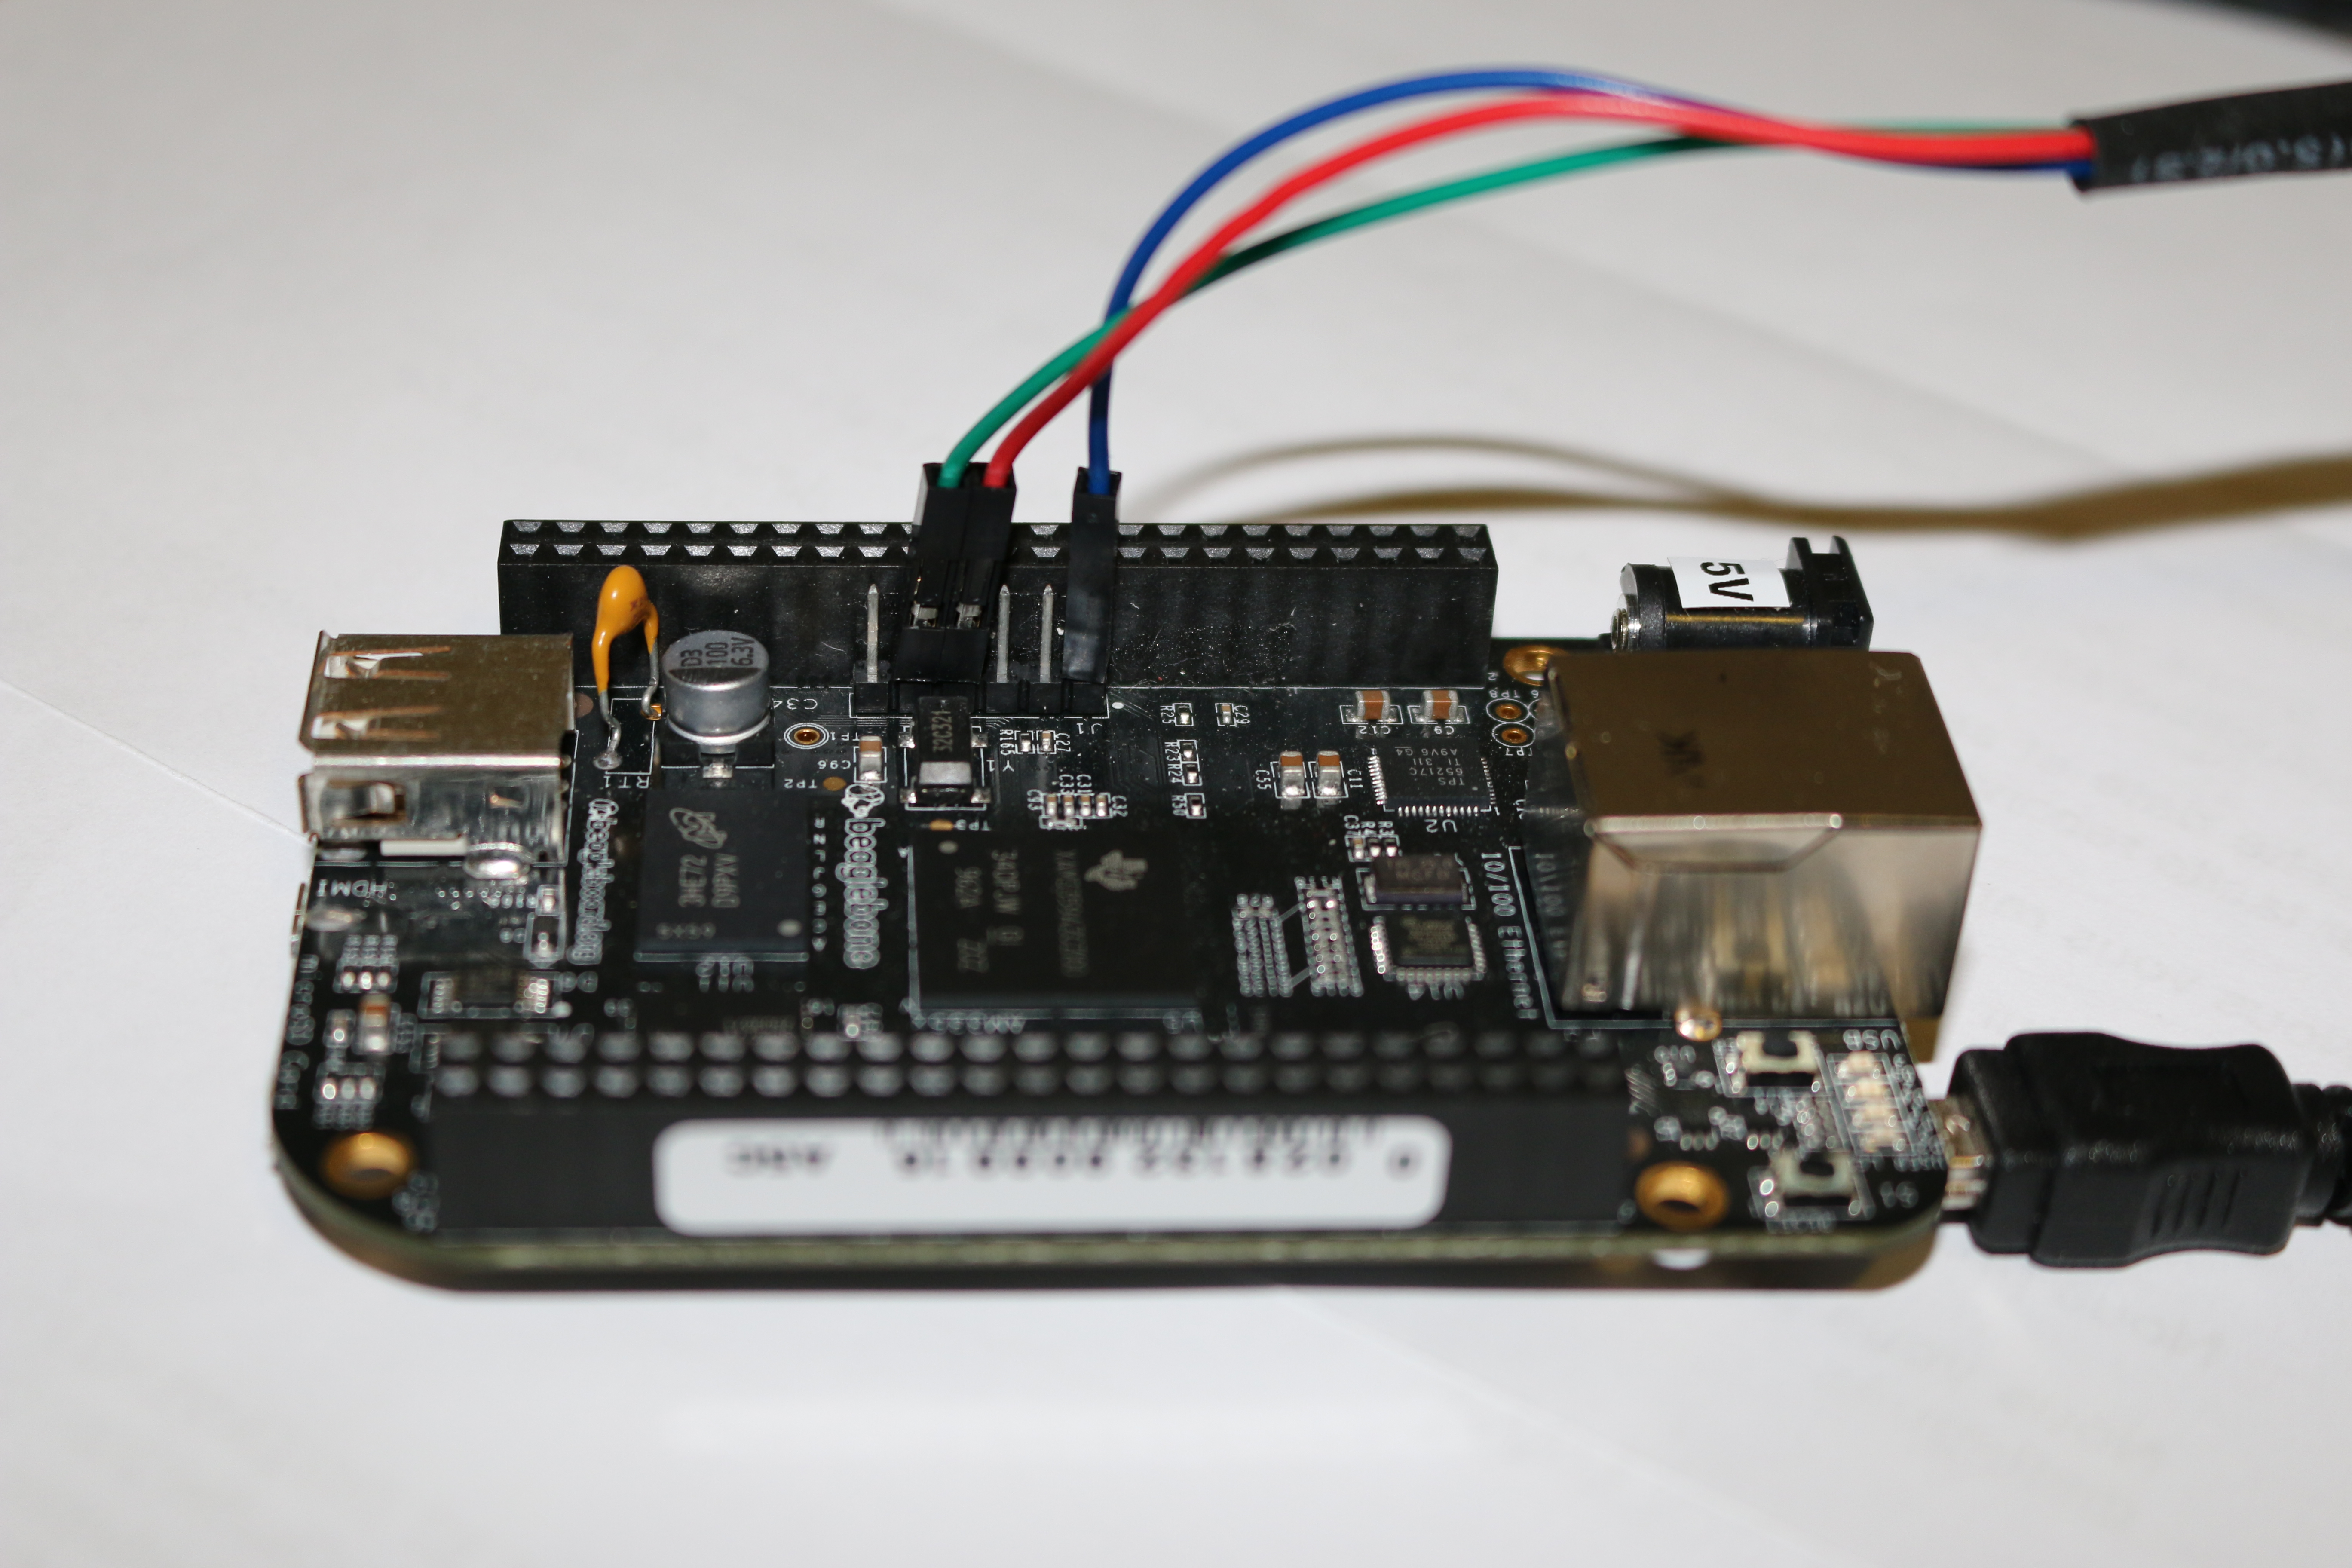
\includegraphics[width=8cm]{common/beaglebone-black-serial-connection.jpg}
\end{center}

Once the USB to Serial connector is plugged in, a new serial port
should appear: \code{/dev/ttyUSB0}.

You can also see this device appear by looking at the output of
\code{sudo dmesg}.

To communicate with the board through the serial port, install a
serial communication program, such as \code{picocom}:

\bashcmd{$ sudo apt install picocom}

If you run {\tt ls -l \hosttty}, you can also see that only
\code{root} and users belonging to the \code{dialout} group have
read and write access to the serial console. Therefore, you need
to add your user to the \code{dialout} group:

\bashcmd{$ sudo adduser $USER dialout}

{\bf Important}: for the group change to be effective, you have to
reboot your computer (at least on Ubuntu 22.04) and log in again.
A workaround is to run \code{newgrp dialout}, but it is not global.
You have to run it in each terminal.

Run {\tt picocom -b 115200 \hosttty}, to start serial
communication on {\tt \hosttty}, with a baudrate of 115200.
If you wish to exit \code{picocom}, press \code{[Ctrl][a]} followed by
\code{[Ctrl][x]}.

There should be nothing on the serial line so far, as the board is not
powered up yet.

It is now time to power up your board by plugging in the mini-USB
(BeagleBone Black case) or micro-USB (BeagleBone Black Wireless case)
cable supplied by your instructor to your PC.

See what messages you get on the serial line. You should see U-boot
start on the serial line, if there was a valid U-Boot and SPL on the board's eMMC.

\section{Compiling U-Boot and SPL}

Download U-Boot:

\begin{bashinput}
$ git clone https://gitlab.denx.de/u-boot/u-boot
$ cd u-boot
$ git checkout v2023.04
\end{bashinput}

Get an understanding of U-Boot's configuration and compilation steps
by reading the \code{README} file, and specifically the {\em Building
the Software} section.

Basically, you need to:

\begin{enumerate}

\item Specify the cross-compiler prefix
(the part before \code{gcc} in the cross-compiler executable name):
\bashcmd{$ export CROSS_COMPILE=arm-linux-}

\item Run \inlinebash{$ ls configs/ | grep am335} to see all predefined
      configurations. The one that supports our board is not obvious:
      it's \code{am335x_evm_defconfig} and not
      \code{am335x_boneblack_vboot_defconfig} which is only for {\em
      verified boot} on BeagleBone Black.
\item So, run \inlinebash{$ make am335x_evm_defconfig}.

\item Now that you have a valid initial configuration, you can now
  run \inlinebash{$ make menuconfig} to further edit your bootloader features.

Here, though, the default configuration works fine for our needs,
so no change is necessary.

Install the following packages which should be needed to compile U-Boot for
your board:

\begin{bashinput}
$ sudo apt install libssl-dev device-tree-compiler swig \
       python3-distutils python3-dev python3-setuptools
\end{bashinput}

\item Finally, depending on your board, run
  \bashcmd{make DEVICE_TREE=am335x-boneblack}
  or \bashcmd{make DEVICE_TREE=am335x-boneblack-wireless}
  which will build U-Boot
  \footnote{You can speed up the
  compiling by using the \code{-jX} option with \code{make}, where X
  is the number of parallel jobs used for compiling. Twice the
  number of CPU cores is a good value.}.
  The \code{DEVICE_TREE} variable specifies the specific
  Device Tree that describes our hardware board.
  Alternatively, if you wish to run just \code{make},
  specify our board's device tree name on
  \code{Device Tree Control} $\rightarrow$ \code{Default Device Tree for DT Control}
  option.
\end{enumerate}

\section{Preparing a bootable micro-SD card}

The TI romcode will look for an \code{MLO} ({\em MMC Load})
file in a FAT partition on an SD card. This is precisely what U-Boot
compiled for us, together with the U-Boot binary (\code{u-boot.img}).

Let's prepare an SD card with such a partition.

Plug the SD card your instructor gave you on your workstation. Type
the \code{sudo dmesg} command to see which device is used by your
workstation. In case the device is \code{/dev/mmcblk0}, you will see
something like

\begin{verbatim}
[46939.425299] mmc0: new high speed SDHC card at address 0007
[46939.427947] mmcblk0: mmc0:0007 SD16G 14.5 GiB
\end{verbatim}

The device file name may be different (such as \code{/dev/sdb}
if the card reader is connected to a USB bus (either internally
or using a USB card reader).

In the following instructions, we will assume that your SD card is
seen as \code{/dev/mmcblk0} by your PC workstation.

Type the \code{mount} command to check your currently mounted
partitions. If SD partitions are mounted, unmount them:

\bashcmd{$ sudo umount /dev/mmcblk0p*}

We will erase the existing partition table by simply zero-ing the
first 16 MiB of the SD card:

\bashcmd{$ sudo dd if=/dev/zero of=/dev/mmcblk0 bs=1M count=16}

Now, let's use the \code{cfdisk} command to create the first partition
that we need to boot the board:
we are going to use:

\bashcmd{$ sudo cfdisk /dev/mmcblk0}

If \code{cfdisk} asks you to \code{Select a label type}, choose
\code{dos}. This corresponds to traditional partitions tables that DOS/Windows
would understand. \code{gpt} partition tables are needed for disks bigger
than 2 TB.

In the \code{cfdisk} interface, delete existing partitions, then
create only one primary partition, starting from the beginning
following properties:

\begin{itemize}
\item Size: 64MB big
\item Type: \code{W95 FAT32 (LBA)} (\code{c} choice)
\item Bootable flag enabled
\end{itemize}

Press \code{Write} when you are done.

We will create further partitions in a later lab, when we need them.

To make sure that partition definitions are reloaded on your
workstation, remove the SD card and insert it again.

Now create a FAT32 filesystem on this new partition:
\footnote{Ubuntu uses version 4.2 of \code{mkfs.vfat} and the FAT
generated by this version of the command is incompatible with what
the TI AM335x romcode expects. Passing the \code{-a} option
a workaround described on on a \href{https://bootlin.com/blog/workaround-for-creating-bootable-fat-partition-for-beagle-bone-am335x-on-recent-distros/}
{Bootlin blog post}.}
\begin{bashinput}
sudo mkfs.vfat -a -F 32 -n boot /dev/mmcblk0p1
\end{bashinput}

You can now make your workstation automatically mount this
partition by removing the SD card and plugging it back. It should
now be mounted on \code{/media/$USER/boot}.

Now, copy the \code{MLO} and \code{u-boot.img} files to the SD card:
\begin{bashinput}
cp MLO u-boot.img /media/$USER/boot/
sudo umount /media/$USER/boot/
\end{bashinput}

\section{Testing U-Boot}

Insert the SD card in the board slot. To boot the board on the external micro-SD
card, you need to hold the \code{USER} button close to the USB host
port, and then power-up or reset the board. You can then release the
\code{USR} button.

This seems like a very inconvenient way of booting the board, but
the selection of attempting to boot from the external micro-SD card
remains active across resets, until the board is ultimately powered off.
So, you will just need to use the button a few times during the course.

If this is too inconvenient for you, you could use U-Boot on the
external micro-SD card to flash a new version of U-Boot on the internal
eMMC. This would allow you to boot without an external micro-SD card.

Here's what you should get on the serial line:

\begin{verbatim}
U-Boot SPL v2023.04 (Jul 06 2023 - 10:47:22 +0100)
Trying to boot from MMC1


U-Boot v2023.04 (Jul 06 2023 - 10:47:22 +0100)

CPU  : AM335X-GP rev 2.1
Model: TI AM335x BeagleBone Black
DRAM:  512 MiB
Core:  160 devices, 18 uclasses, devicetree: separate
WDT:   Started wdt@44e35000 with servicing (60s timeout)
NAND:  0 MiB
MMC:   OMAP SD/MMC: 0, OMAP SD/MMC: 1
Loading Environment from FAT... Unable to read "uboot.env" from mmc0:1...
<ethaddr> not set. Validating first E-fuse MAC
Net:   eth2: ethernet@4a100000, eth3: usb_ether
Hit any key to stop autoboot:  0
=>
\end{verbatim}

Make sure that the version and compile date are right. Otherwise, try
again, because this means that you booted on the internal eMMC.

In U-Boot, type the \code{help} command, and explore the few commands
available.

\subsection{Adding a new command to the U-Boot shell}

Check whether the \code{config} command is available. This command
allows to dump the configuration settings U-Boot was compiled from.

If it's not, go back to U-Boot's configuration and enable it.

Re-run the build of U-Boot, and update the bootloader on the SD card
and test that the command is now available and works as expected.

\subsection{Playing with the U-Boot environment}

Display the U-Boot environment using \code{printenv}.

Set a new U-Boot variable \code{foo} to a value of your choice, using
\code{setenv}, and verify it has been set. Reset the board, and check
if \code{foo} is still defined: it should not.

Now repeat this process, but before resetting the board, use
\code{saveenv}. After the reset, check the \code{foo} variable is
still defined.

Now reset the environment to its default settings using \code{env
  default -a}, and save these changes using \code{saveenv}.

\section{Setting up networking}

The next step is to configure U-boot and your workstation to let your
board download files, such as the kernel image and Device Tree Binary
(DTB), using the TFTP protocol through a network connection.

As this course supports both the BeagleBone Black and BeagleBone Black
Wireless boards, we're keeping things simple by using Ethernet over USB
device as this works for both boards (as the Wireless board has no
native Ethernet port). So, networking will work through the USB device
cable that is already used to power up the board.

{\bf Caution}: For the following to work, make sure that your board
is powered by a USB port on your PC. Otherwise, networking over USB
cannot work.

\subsection{Network configuration on the target}

Let's configure networking in U-Boot:

\begin{itemize}
  \item \code{ipaddr}: IP address of the board
  \item \code{serverip}: IP address of the PC host
\end{itemize}

\begin{ubootinput}
=> setenv ipaddr 192.168.0.100
=> setenv serverip 192.168.0.1
\end{ubootinput}

Of course, make sure that this address belongs to a separate network
segment from the one of the main company network.

We also need to configure Ethernet over USB device:
\begin{itemize}
  \item \code{ethprime}: controls which interface gets used first
  \item \code{usbnet_devaddr}: MAC address on the device side
  \item \code{usbnet_hostaddr}: MAC address on the host side
\end{itemize}

\begin{ubootinput}
=> setenv ethprime usb_ether
=> setenv usbnet_devaddr f8:dc:7a:00:00:02
=> setenv usbnet_hostaddr f8:dc:7a:00:00:01
\end{ubootinput}

To make these settings permanent, save the environment:

\begin{ubootinput}
=> saveenv
\end{ubootinput}

\subsection{Network configuration on the PC host}

To configure your network interface on the workstation side, we need
to know the name of the network interface connected to your board.

Note that when the board is waiting at the U-Boot prompt, no network
interface will show up on the workstation side. It is only when U-Boot
is actively executing a network-related command (such as \code{ping}
or \code{tftp}) that it brings up the USB network connection.

From the board, run \code{ping 192.168.0.1}, and while the \code{ping}
command is running, you should see on your workstation a new network
interface named \code{enx<macaddr>}. Given the value we gave to
\code{usbnet_hostaddr}, it will therefore be
\code{enxf8dc7a000001}. Note that pinging the board from your PC will
not work: when U-Boot is waiting at its prompt, it is not able to
reply to ping requests.

Then, instead of configuring the host IP address from NetWork Manager's
graphical interface, let's do it through its command line interface,
which is so much easier to use:

\bashcmd{nmcli con add type ethernet ifname enxf8dc7a000001 ip4 192.168.0.1/24}

\section{Setting up the TFTP server}

Let's install a TFTP server on your development workstation:

\begin{verbatim}
sudo apt install tftpd-hpa
\end{verbatim}

You can then test the TFTP connection. First, put a small text file in
the directory exported through TFTP on your development
workstation. Then, from U-Boot, do:

\begin{ubootinput}
=> tftp %\zimageboardaddr% textfile.txt
\end{ubootinput}

The \code{tftp} command should have downloaded the
\code{textfile.txt} file from your development workstation into
the board's memory at location {\tt \zimageboardaddr}\footnote{
This location is part of the board DRAM. If you want
to check where this value comes from, you can check the SoC
datasheet at
\url{https://www.ti.com/lit/ug/spruh73q/spruh73q.pdf}.
It's a big document (more than 5,000 pages). In this document, look
for \code{ARM Cortex-A8 Memory Map} and you will find the SoC memory map.
You will see that the address range for the memory controller
({\em EMIF0 SDRAM})
starts at the address we are looking for.
You can also try with other values in the RAM address range.}.

You can verify that the download was successful by dumping the
contents of the memory:

\begin{ubootinput}
=> md %\zimageboardaddr%
\end{ubootinput}

We will see in the next labs how to use U-Boot to download, flash and
boot a kernel.


\section{Rescue binaries}

If you have trouble generating binaries that work properly, or later
make a mistake that causes you to lose your bootloader binaries, you
will find working versions under \code{data/} in the current lab
directory.
